\section{Theoretical Introduction}

\subsection{Social Homophily}

\epigraph{``People love those who are like themselves.''}{\textit{Rhetoric \\ Aristotle}}

Similarity breeds connection\cite{mcpherson2001birds}. People have several visible characteristics, such as age, gender, and socioeconomic status, for which contact between people with similar properties occurs at a higher rate than between dissimilar people.

There are two overall types of homophily that can be distriguished in groups\cite{lazarsfeld1954}: \textit{status homophily}, in which similarity is based on status, and \textit{value homophily}, which is based on values, attitudes, and beliefs. Status homophily, a part of which is the main study of this thesis, includes the major sociodemographic dimensions that stratify society --- ascribed characteristics like race, ethnicity, sex, or age, and acquired characteristics like religion, education, occupation, and behaviour patterns.

\subsubsection{Age Homophily}

One of the most common homophily patterns in human relations is related to the people's ages\cite{ugander2011}\cite{mcpherson2001birds}. This result is expected because of the many societal reasons that explain the homophily: schools tend to group people according to age into the sane classroooms, work opportunities tend to be clustered into age groups, which affects work environments and neighbourhood composition, and people have a strong tendency to confide in someone of one's own age.

This correlation has a waterfall effect. Since this kind of homophily is present since early into people's life, the producded connections are closer, longer lived, have a larger number of exchanges, and tend to be more personal than other kinds of connections. Indeed, people have a strong tendency to confide in someone of one's own age\cite{mcpherson2001birds}\todo{find better cite}.

There's an interesting exception to this homophily: there is a significant number of connections between parents and their younger children\cite{sarraute2014}\todo{check this}. This exception is addressed later in this paper.

\subsubsection{Gender Homophily}

Lorem ipsum dolor sit amet.

\subsection{Spearman's Coefficient}

Spearman's Rank Correlation Coefficient (also known as Spearman's rho) is a nonparametric measure of rank correlation which measures how well the relationship between two variables can be described using a monotonic function\cite{statistical_analysis}. Unlike Pearson's Correlation Coefficient, which measures lineal relationship between variables, Spearman's Coefficient uses the \emph{rank} of the variables in its calculations; therefore is measures its monotonicity.

For a sample of size \( n \) with scores \( X_i \) and \( Y_i \), the Spearman Coefficient \( r_s \) is defined as

\begin{equation}
r_s = \mathlarger{\rho}_{\rank(X) \rank(Y)} = \frac{\operatorname{cov}(\rank(x), \rank(y))}{\sigma_{\rank(X)} \sigma_{\rank(Y)}}
\label{spearman}
\end{equation}

Where \( \rho_{a,b} \) denotes the Pearson correlation between the variables \( a \) and \( b \). This value will be close to 1 when the variables are directly monotonic, close to -1 when they are inversely monotonic, and close to 0 when there is no tendency for either variable to increase or decrease when the other increases.

\subsection{Bayesian Inference}

\epigraph{``Given the number of times in which an unknown event has happened and failed: required the chance that the probability of its happening in a single trial lies somewhere between any two degrees of probability that can be named.''}{\textit{An Essay towards solving a Problem in the Doctrine of Changes~\cite{bayes1763} \\ Thomas Bayes}}

This work uses a Bayesian approach to statistics instead of the usual Frequentist approach. In the Frequentist point of view, parameters are fixed and unknown: hypotheses are either true or false, and they cannot be described with a probability. In the Bayesian approach, anything unknown is described with a probability distribution since uncertainty must be described by probability~\cite{mackay}.

\subsubsection{Bayes Theorem}

The base of \emph{Bayesian Inference} is \emph{Bayes' Theorem}, presented in Equation~\ref{eq:bayes}, which describes the probability of an event base on prior knowledge of conditions that may be related to it~\cite{gelman2003}.

\begin{equation}
\label{eq:bayes}
	P \left( H \mid E \right) = \frac{P \left( E \mid H \right) \cdot P \left( H \right)}{P \left( E \right)}
\end{equation}

Each one of the terms in Equation~\ref{eq:bayes} has a different definition and interpretation.

\begin{itemize}
	\item $P \left( H \mid E \right)$, the \textbf{Posterior Probability} is the conditional probability that is assigned after the relevant evidence is taken into account.
	\item $P \left( H \right)$, the \textbf{Prior Probability}, expresses the assumptions made on the problem before the experiments. While these assumptions will be subjective, the same thing can be said about the other probabilities in this model.
	\item $P \left( E \mid H \right)$, the \textbf{Likelihood}, is the degree of belief in $E$ given that $H$ is true. In most real world problems, this tends to be easier to define than the \emph{Prior}.
	\item $P \left( E \right)$, the \textbf{Marginal Likelihood}, as the likelihood function where some parameter variables were marginalized. It's used as a normalizing constant to that the \emph{Posterior Probability} integrates to 1, thus making it a valid probability. Since it's constant on the perspective of $H$, it's usually ignored when taking proportionality, as in Equation~\ref{eq:bayes_propto}.
\end{itemize}

It can be proven in a simple way by using basic theorems of the probability, as seen in Equation~\ref{eq:bayes_proof}.

\begin{equation}
\label{eq:bayes_proof}
\begin{aligned}
	P \left( H \cap E \right)
	&= P \left( H \mid E \right)P \left( E \right) \\
	&= P \left( E \mid H \right)P \left( H \right) \\
	P \left( H \mid E \right) P \left( E \right) &= P \left( E \mid H \right) P \left( H \right) \\
	P \left( H \mid E \right) &= \frac{P \left( E \mid H \right) P \left( H \right)}{P \left( E \right)}
\end{aligned}
\end{equation}

Most of the equations presented in this section deal with continuous probabilities, which by definition must integrate to 1~\cite{kolmogrov1956}. Therefore, the theorem is usually used in the version presented in Equation~\ref{eq:bayes_propto}, which defines the proportionality of the \emph{Posterior}.

\begin{equation}
\label{eq:bayes_propto}
	P \left( H \mid E \right) \propto P \left( E \mid H \right) \cdot P \left( H \right)
\end{equation}

\begin{figure}
\centering
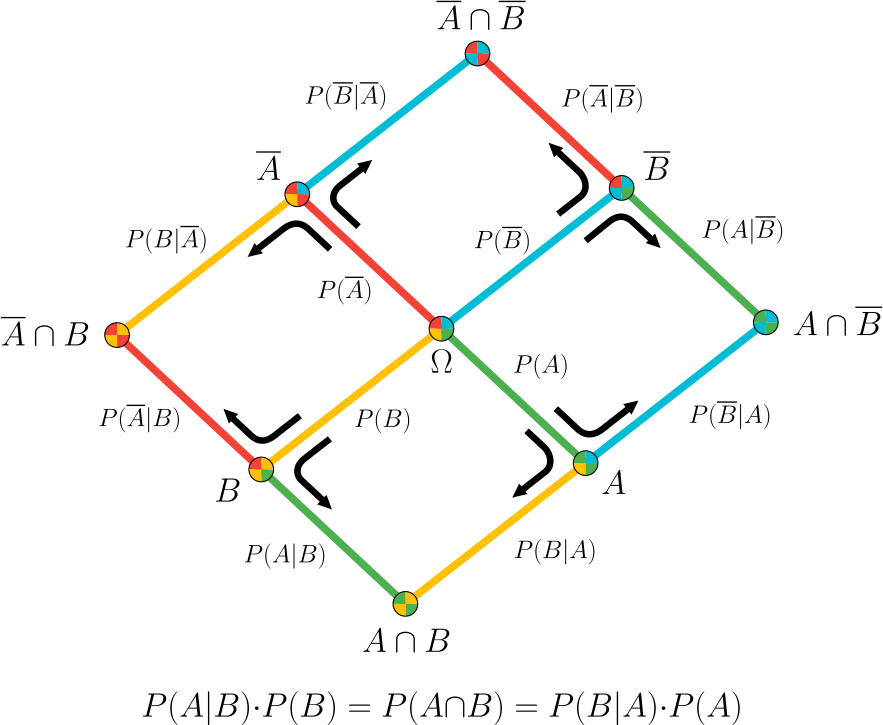
\includegraphics[width=.7\textwidth]{figures/Bayes_Theorem.png}
\caption{Graphical visualization of \emph{Bayes Theorem} between two probabilities $A$ and $B$ by the superposition of two decision trees starting in hypothesis space $\Omega$.}
\label{fig:Bayes_Theorem}
\end{figure}

\subsubsection{Conjugate Priors}
\label{subsec:conjugate}

For a single problem there may be many different possible \emph{Prior Probabilities}, which can be defined depending on the approach taken on defining the model to represent different measures of knowledge and certainty about the data\footnotemark{}. In particular, if the prior is less informative then the posterior is more likely to be determined by the data.

\footnotetext{An extreme case is the \emph{Jeffreys Prior}, used to express total ignorance about the data~\cite{jeffreys453}.}

A simple way to choose a correct prior is using a \emph{Conjugate Prior}. A distribution $P \left( H \right)$ is \emph{Conjugate} to $P \left( H \mid E \right)$ if multiplying the two distributions together and normalizing the results in another distribution has the form as $P \left( H \right)$\maybe{Check this}.

The \emph{Conjugate Prior} has some philosophical significance in the context of \emph{Bayesian Estimator}. In the practical case, the \emph{Prior Probability} contains more or less information compared to the \emph{Posterior Probability} depending on the amount of data seen. In particular, if the experiment has seen little data, a single datapoint can influence your beliefs significantly. On the other hand, if the experiment has a lot of data, then one single extra datapoint shouldn't influence them as much~\cite{gelman2003}.

\subsection{The Beta Distribution}
\label{subsec:beta}

The \emph{Beta Distribution} is a family of continuous probability distributions defined in the interval $\left[ 0, 1 \right]$ which is parametrized by two shape parameters, $\alpha$ and $\beta$.

The distribution can be used to model the behaviour of \emph{Random Variables} limited to intervals of a finite length. It is often used as a statistical function to model unknown data from a known sample, such as allele frequencies in population genetics~\cite{Balding1995}, Malaysian sunshine data~\cite{Sulaiman1999573}, and heterogeneity in the probability of HIV transmission~\cite{SIM:SIM4780080110}.

In the context of \emph{Bayesian Inference}, the \emph{Beta Distribution} is the \emph{Conjugate Prior} of the \emph{Binomial Distribution}, which allows us to describe initial knowledge concerning probability of success of a single bi-variate distribution. In layman terms, this allows us to know what is the distribution of the continuous $p$ parameter of a binomial distribution for which we have $\alpha$ positive and $\beta$ negative samples.

\subsubsection{Probability Density Function}

Given a variable $0 \leq x \leq 1$, which represents the unknown probability of having a \emph{Positive Sample} from the distribution, and the shape parameters $\alpha > 0$ and $\beta > 0$, the \emph{Probability Density Function} of the beta distribution can be described as in Equation~\ref{eq:beta_pdf}, where $\kappa$ represents some constant.

\begin{equation}
\label{eq:beta_pdf}
\begin{aligned}
f\left(x; \alpha, \beta\right) &= \kappa \cdot x^{\alpha - 1} {\left( 1 - x \right)}^{\beta - 1} \\
&= \dsfrac{x^{\alpha - 1} {\displaystyle \left( 1 - x \right)}^{\beta - 1}}{\int^1_0 {u^{\alpha - 1} {\left( 1 - u \right)}^{\beta - 1} du}} \\
&= \dsfrac{\Gamma \left( \alpha + \beta \right)}{\Gamma \left( \alpha \right) \Gamma \left( \beta \right)} \cdot x^{\alpha - 1} {\left( 1 - x\right)}^{\beta - 1} \\
&= \dsfrac{1}{\Beta \left(\alpha, \beta\right)} \cdot x^{\alpha - 1} {\left(1 - x\right)}^{\beta - 1}
\end{aligned}
\end{equation}

\begin{equation}
\label{eq:beta_function}
\Beta\left(\alpha, \beta\right) = \frac{\Gamma\left(\alpha + \beta\right)}{\Gamma\left(\alpha\right) \Gamma\left(\beta\right)}
\end{equation}

\Cref{eq:beta_function}, describes the \emph{Beta Function}, which is related to the \emph{Gamma Function} and describes a similar pattern~\cite{thegammafunction}.

Regarding this thesis, the \emph{Beta Distribution} will be used to model a real life problem in Section~\ref{sec:inference_methodology}. In this problem, both $\alpha \in \mathbb{N}$ and $\beta \in \mathbb{N}$, so the \emph{Beta Function} can be simplified using the identity $\left( x - 1 \right)! = \Gamma \left( x \right)$ as shown in Equation~\ref{eq:beta_int}.

\begin{equation}
\label{eq:beta_int}
\Beta(\alpha, \beta) = \frac{(\alpha + \beta - 1)!}{(\alpha - 1)! \cdot (\beta - 1)!}
\end{equation}

Additionally, the \emph{Beta Function} can be generalized into the \emph{Incomplete Beta Function} for some parameter $x$ as in Equation~\ref{eq:incomplete_beta}. This function is, confusingly, also represented with the greek letter $\Beta$; to ease comprehension this thesis will refer to it as $\Betainc$.

\begin{equation}
\label{eq:incomplete_beta}
\Betainc(x; \alpha, \beta) = \int_0^x {t^{\alpha - 1} {(1 - t)}^{\beta - 1} dt}
\end{equation}

As we get more data from the sampling, the \emph{Beta distribution} turns more concenteated towards the actual \( \theta \) and its shapes resembles more a normal curve, as can be seen in \Cref{fig:betagraph}. This represents the increased certainty which comes from the aquired knowledge of the problem.

\begin{figure}
\centering
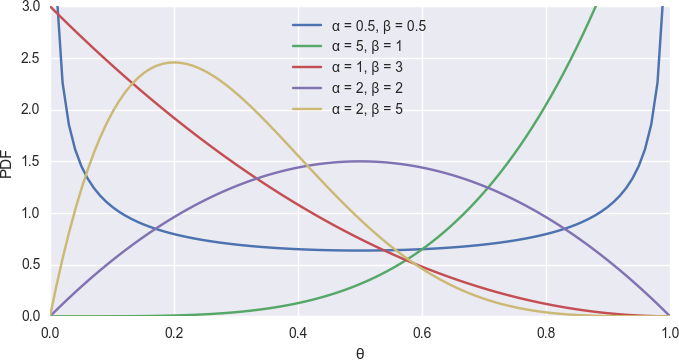
\includegraphics[width=\textwidth]{figures/beta.png}
\caption{Beta distribution with different parameters}
\label{fig:betagraph}
\end{figure}

\subsubsection{Cumulative Distribution Function}

The \emph{Cumulative Distribution Function} of the \emph{Beta Distribution} is defined in Equation~\ref{eq:beta_cdf_formula}.

\begin{gather}
\begin{gathered}
\label{eq:beta_cdf}
X \sim \Betadist \left( \alpha, \beta \right) \\
F \left( x; \alpha, \beta \right) = P \left( X \leq x \right)
\end{gathered} \\
\label{eq:beta_cdf_formula}
\begin{aligned}
F \left( x; \alpha, \beta \right)  &= \int_0^x f \left( t; \alpha, \beta \right) dt \\
&= \int_0^x {\frac{1}{\Beta \left( \alpha, \beta \right)} t^{\alpha - 1} {\left( 1 - t \right)}^{\beta - 1} dt} \\
&= \frac{1}{\Beta \left( \alpha, \beta \right)} \cdot \int_0^x {t^{\alpha - 1} {\left( 1 - t \right)}^{\beta - 1} dt} \\
&= \frac{\Betainc \left( x; \alpha, \beta \right)}{\Beta \left( \alpha, \beta \right)}
\end{aligned}
\end{gather}

$F$ is also known as the \emph{Regularized Incomplete Beta Function}, represented as $I_x(\alpha, \beta)$. This function is related to the \emph{Cumulative Distribution Function} of the \emph{Binomial Distribution}, as shown in Equation~\ref{eq:incomplete_beta_binomial}.

\begin{equation}
\label{eq:incomplete_beta_binomial}
\begin{gathered}
X \sim \Betadist \left( n, p \right)  \\
P \left( X \leq k \right)  = I_{1 - p} \left( n - k, k + 1 \right)
\end{gathered}
\end{equation}

\subsubsection{Inverse Cumulative Distribution Function}
\label{subsec:beta_ppf}

The problems solved in this thesis require the use of the \emph{Inverse Cumulative Distribution Function} (also known as the \emph{Quantile Function} or the \emph{Percent-Point Function}) of the \emph{Beta Distribution}, which returns a value such $x$ that meets the expression in Equation~\ref{eq:beta_cdf} is equal to some value $p$. It can also be expressed as in Equation~\ref{eq:quantile_function}.

\begin{equation}
\label{eq:quantile_function}
Q \left( p \right)  = \inf \left\{ x \in \mathbb{R} \mid p \leq F \left( x \right) \right\}
\end{equation}

Like with the \emph{Cumulative Distribution Function}, there is no closed form formula for expressing its inverse~\cite{kippingexoplanets2013}. However, there are fast and accurate ways of computing it using either \emph{Interval~Halving} or \emph{Newton's~Method}, such as the \texttt{incbi} implementation in the \emph{Cephes} library~\cite{cephes} which is use in this thesis via a wrapper from \texttt{sklearn}, as explained in Section~\ref{subset:machine_properties}.

\subsubsection{The Beta-Binomial Model}
\label{subsec:betabin}

In the \emph{Beta-Binomial Model} compromises a family of discrete probability distributions similar to the \emph{Binomial Distribution}, with the important difference that, instead of each trial having a constant probability of success, that probability is random and follows the \emph{Beta Distribution}~\cite{schervish1996statistics}.

Given a binary experiment which is run $n$ times, and the probability of success of any of those experiment is some constant $\theta$, the \emph{Probability Distribution} of the amount of successes $k$ can be modelled with a \emph{Binomial Distribution}, as shown in Equation~\ref{eq:betabin_binomial}.

\begin{equation}
\label{eq:betabin_binomial}
\begin{gathered}
	k \mid n, \theta \sim \Binomial \left( \theta, n \right) \\
	P \left( k = x \mid n, \theta \right) = \binom{n}{k} \cdot \theta^k {\left( 1 - \theta \right)}^{n - k}
\end{gathered}
\end{equation}

$\theta$ is a random continuous probability distribution, which is defined using the \emph{Beta Distribution} in Equation~\ref{eq:betabin_beta}.

\begin{equation}
\label{eq:betabin_beta}
\begin{gathered}
	\theta \mid \alpha, \beta \sim \Beta \left( \alpha, \beta \right) \\
	P \left( \theta \mid \alpha, \beta \right) = \frac{1}{\Beta \left( \alpha, \beta \right)} \cdot \theta^{\alpha - 1} {\left( 1 - \theta \right)}^{\beta - 1}
\end{gathered}
\end{equation}

Once the binary experiment is run, the model has additional information which may change the distribution of $\theta$. This can be modelled as a \emph{Posterior Distribution} using \emph{Bayes Theorem}~\cite{betabinomialcmu}.

\begin{equation}
\label{eq:betabin_bayes}
\begin{aligned}
	P \left( \theta \mid n, k, \alpha, \beta \right)
	&= \frac{P \left( k \mid n, \theta \right) P \left( \theta \mid n, \alpha, \beta \right)}{P \left( k \mid n, \alpha, \beta \right)} \\
	&\propto P \left( k \mid n, theta \right) P \left( \theta \mid n, \alpha, \beta \right) \\
	&= P \left( k \mid n, \theta \right) P \left( \theta \mid \alpha, \beta \right) \\[1em]
	P \left( \theta \mid n, k, \alpha, \beta \right)
	&= \binom{n}{k} \theta^k {\left( 1 - \theta \right)}^{n - k} \cdot \frac{1}{\Beta \left( \alpha, \beta \right) } \theta^{\alpha - 1} {\left( 1 - \theta \right)}^{\beta - 1} \\
	&\propto \theta^k {\left( 1 - \theta \right)}^{n - k} \cdot \theta^{\alpha - 1} {\left( 1 - \theta \right)}^{\beta - 1} \\
	&= \theta^{k + \alpha - 1} {\left( 1 - \theta \right)}^{n - k + \beta - 1}
\end{aligned}
\end{equation}

This is exactly the same function as the one in Equation~\ref{eq:betabin_beta}. That is, the \emph{Posterior Distribution} of this model is also a \emph{Beta Distribution}.

\begin{equation}
\label{eq:betabin_posteriorbeta}
	\theta \mid k, n, \alpha, \beta \sim \Betadist \left( \alpha + k, \beta + n - k \right)
\end{equation}

This way it's possible to see that the \emph{Beta Distribution} has the properties of a \emph{Conjugate Prior Distribution} seen in Section~\ref{subsec:conjugate} to the \emph{Binomial Likelihood}. This makes it extremely desiderable for \emph{Bayesian Analysis}, and for this reason it's used as the main model of this thesis. This is seen in more detail Section~\ref{subsec:modelling_users}.

\subsection{Machine Learning Validation Metrics}
\label{subsec:mlmetrics}

In the following subsections we present the outline of several supervised machine learning algorithms which are used to compare the Bayesian method to a more realistic baseline. First, we'll present several ways to validate the different algorithms when applied to the data. In the following section, we'll present many of the algorithms used for comparison.

Given a set of fatures $Z$, all of which belong to members of a population which belong to a certain category, and a random subset of those features $X \subseteq Z$ whose category $y$ is known, the models should be trained with $X$ and $y$ in order to correctly predict the values corresponding to all the features in $Z$. Since those values are unknown validation of the output is impossible; therefore, we validate the model using the known values in $X$ and $y$.

There are many metrics that can be used to measure the performance of a classifier or a predictor~\cite{binaryevaluation}; different fields have different preferences due to different goals. In this section, we present many metrics to evaluate different results that are commonly used in the area of mobile phone data analysis~\cite{oskardottir2016}.

\subsubsection{Classification of individual results}

Once we define out classifier $g$ and run it against a matrix\maybe{Set?} of features\maybe{Should I explain train/test split before this subsubsection?}, we get a predicted result $\ypred$ which, when compared to the actual result $\ytrue = y$, can be classified as the one in Table~\ref{tab:confusion}.

\begin{table}[h]
\begin{tabularx}{\textwidth}{| c | X | X X |}
\hline

& & \multicolumn{2}{c|}{\textbf{Predicted Condition}} \\
& Total Population &
\makecell{Condition Positive} &
\makecell{Condition Negative} \\ \hline

\multirow{2}{5em}{\textbf{True Condition}} &
Condition Positive &
\cellcolor{OrangeRed} \makecell{\textbf{True Positive}} &
\cellcolor{CadetBlue} \makecell{\textbf{False Negative} \\ (Type II error)} \\


& Condition Negative &
\cellcolor{CadetBlue} \makecell{\textbf{False Positive} \\ (Type I Error)} &
\cellcolor{OrangeRed} \makecell{\textbf{True Negative}} \\ \hline

\end{tabularx}
\caption[caption]{Confusion Table, showing different classifications of an individual prediction. \\ True and False Positives ($\TP$/$\FP$) refer to the number of predicted positives that were correct/incorrect, and similarly for True and False Negatives ($\TN$/$\FN$).}
\label{tab:confusion}
\end{table}

Additionally, this table can be easily seen in a graphical way in figure~\ref{fig:truefalsenegativepositive}.

\begin{figure}
\centering
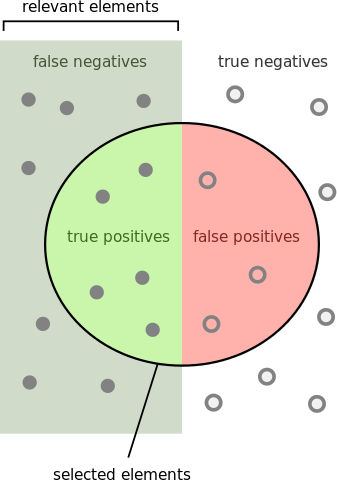
\includegraphics[width=15em]{figures/TrueFalseNegativePositive.png}
\caption{Visual explanation of \emph{Precision} and \emph{Recall}}
\label{fig:truefalsenegativepositiv}
\end{figure}

\subsubsection{Precision and Recall}
\label{subsec:precisionrecall}
\emph{Precision} denotes the proportion of predicted positive cases that are correctly real positive. Trying to maximize this would allow us to adjust a particular predictor so that the majority of the predicted cases are actually positive. Conversely, \emph{recall} is the proportion of real positive cases that are correctly predicted positive, and maximizing it would allow us to adjust a predictor so that the majority of positive cases are predicted.

\begin{equation}
\begin{split}
\Precision = \TPA &= \frac{\TP}{\TP + \FP} \\
\Recall = \TPR &= \frac{\TP}{\TP + \FN}
\end{split}
\label{precisionrecall}
\end{equation}

These two measures and their combinations focus only on the positive examples and predictions, althrough between them they capture some information about the rates and kind of errors made\cite{binaryevaluation}. While the \emph{recall} has been shown to have a major weight in working with machine translation\cite{fraser2007}, they aren't particularly useful to use alone since they don't take into account many factors of the prediction\cite{binaryevaluation}.

\subsubsection{Inverse~Precision and Inverse~Recall}

As a corollary of the previous metrics, we can add metrics that measure the proportion of real negative cases that are correctly predicted negative, referred as the \emph{Inverse~Recall}, and the proportion of predicted negatives that are real negatives, referreed as the \emph{Inverse~Precision}\cite{binaryevaluation}. We can see that these are equivalent to finding the \emph{Precision} and \emph{Recall} of the negative category.

\begin{equation}
\begin{split}
\InvPrecision = \TNR &= \frac{\TN}{\FP + \TN} \\
\InvRecall = \TNA &= \frac{\TN}{\FN + \TN}
\end{split}
\label{negativeprecisionrecall}
\end{equation}

\subsubsection{Accuracy}
\label{subsec:accuracy}
The \emph{accuracy}, commonly referred in te context of binary classifiers as \textbf{Rand~Accuracy}\cite{powers15}, is used as a statistical measure of how well a binary classification test identifies or excludes a condition. Unlike the \emph{precision}, it takes into account the negatives, and it's expressible\cite{binaryevaluation} both as a weighted average of \emph{precision} and inverse \emph{precision} or \emph{recall} and \emph{inverse recall}.

\begin{equation}
\Accuracy = \frac{\TP + \TN}{N}
\label{accuracy}
\end{equation}

This can be more simply expressed using the weighted average of either the \emph{Precision} and \emph{Inverse~Precision} or the \emph{Recall} and the \emph{Inverse~Recall}.

\begin{equation}
\begin{split}
\Accuracy &= \left(\TP + \TN\right) \cdot \TPR + \left(\FP + \TN\right) \cdot \TNR \\
&= \left(\TP + \FP\right) \cdot \TPA + \left(\FN + \TN\right) \cdot \TNA
\end{split}
\label{accuracy2}
\end{equation}

\subsubsection{ROC Curve}

A \emph{Receiver Operating Characteristing} graph is a technique for visualizing, organizing, and selecting classifiers based on their performance\cite{fawcett2005}. The curve is created by plotting the \emph{True Positive Rate} against the \emph{False Positive Rate} at various threshold settings.

This allows to compare different classifiers before having to select a particular threshold value for them. In particular, a random classifier will score near the positive diagonal ($\FPR = \TPR$), while a perfect classifier will score in the top left hand corner ($\FPR = 1, \TPR = 0$) and a worst case classifier will score in the bottom right hand corner\footnote{Note that, for any binary classifier, it's trivial to transpose the entire ROC curve (or a part of it) to the other part of the diagonal; therefore the worst ``realistic'' case is the random one}\cite{binaryevaluation}.

\begin{figure}
\todo{Add figure of ROC with AUC}
\caption{A \emph{ROC Curve}, where the \emph{Area Under the Curve} is marked}
\label{fig:roc}
\end{figure}

\subsubsection{Area Under the Curve}
\label{subsec:auc}
The \emph{ROC Curve} allows us to compare classifiers and choose the one which is closer to optimal in some sense. While there are many possible parametrizations, the most common is to minimize the \emph{Area Under the Curve}, which is equal to the probability that a classifier will rank a randomly chosen positive instance higher than a randomly chosen negative one\cite{fawcett2005}. This can be formulated as shown in formula~\ref{eq:auc}.

\begin{equation}
\begin{split}
\AUC &= P\left(X_1 > X_0\right) \\
&= \todo{Something something}
\end{split}
\label{eq:auc}
\end{equation}

\subsubsection{F-measure}
\label{subsec:fmeasure}
The \emph{F-measure} is another measure of a tests accuracy. It considers both the \emph{Precision} and the \emph{Recall} of the test to compute the score. It can be considered the weighted average of both values for some weight $\beta$, where $F_\beta$ reaches the best score 1 when both precision and recall are 1.

\begin{equation}
\begin{split}
F_\beta &= \left( 1 + \beta^2 \right) \cdot \frac{\TPA \cdot \TPR}{\left( \beta^2 \cdot \TPA \right) + \TPR} \\
&= \frac{\left( 1 + \beta^2 \right) \cdot \TP}{\left( 1 + \beta^2 \right) \cdot \TP + \beta^2 \cdot \FN + \FP}
\end{split}
\end{equation}

The most commonly used \emph{F-measure}, $F_1$, measures the \emph{Precision} and \emph{Recall} is thet harmonic mean of the \emph{Precision} and \emph{Recall}. In particular, for an \emph{F-measure} with $\beta > 1$ weights Recall higher than Precision, while with $\beta < 1$ weights Precision higher than Recall.

\section{Supervised Machine Learning Models}
\label{subsec:supervised_machine_learning}

This section presents several \emph{Supervised Machine Learning} models that are used in the paper.

Models are separated into two different groups depending on how they describe the input and output variables.

\begin{description}
	\item[Continuous Models] take a matrix $X \in \mathbb{R}^{n \times f}$ and a vector $y \in \mathbb{R}^n$ of the same height where each element represents the features corresponding to some user and its real value, respectively. Its accuracy is measured according to some function of the result of the regression $\ypred$ and $\ytrue = y$.
	\item[Categorical Models] take a matrix $X \in \mathbb{R}^{n \times f}$ and a vector $y \in \mathbb{S}^n$, for some set of \emph{Categories} $\mathbb{S}$, and predicts the correct category each of the users in $y$ belongs to. Its accuracy is measured according to several metrics which are explained in \cref{subsec:mlmetrics}.
\end{description}

\subsection{Linear Regression}
\label{subsec:linearregression}

A \emph{Linear Regression} is an approach for modeling the relationship between the matrix $X$ and the real vector $y$. While it's possible to predict many variables in what's known as the \emph{Multivariate Linear Regression}~\cite{multivariate1979}, this thesis will focus in the single-dimensional variant.

The regression assumes that the relationship between the sum of some linear combination of the elements of $X$ and $y$ is itself linear. This combination is represented by the variable $\beta$, and the relationship is represented through an unobserved random vector $\varepsilon$ as the \emph{Error Term}.

The model takes the form of \cref{eq:linearregression}.

\begin{gather}
	y = X \beta + \varepsilon \label{eq:linearregression} \\
	\intertext{where}
	\begin{gathered}
		X = \begin{pmatrix} x_1^T \\ x_2^T \\ \vdots \\ x_n^T \end{pmatrix} =
		\begin{pmatrix}
			1 & x_{1 1} & \cdots & x_{1 f} \\
			1 & x_{2 1} & \cdots & x_{2 f} \\
			\vdots & \vdots & \ddots & \vdots \\
			1 & x_{n 1} & \cdots & x_{n f} \\
		\end{pmatrix} \\
		y = \begin{pmatrix} y_1 \\ y_2 \\ \vdots \\ y_n \end{pmatrix}, \;
		\beta = \begin{pmatrix} \beta_0 \\ \beta_1 \\ \vdots \\ \beta_f \end{pmatrix}, \;
		\varepsilon = \begin{pmatrix} \varepsilon_1 \\ \varepsilon_2 \\ \vdots \\ \varepsilon_n \end{pmatrix}
	\end{gathered}
\end{gather}

$\beta$ is a vector with size $f + 1$, where $\beta_0$ is called the \emph{Constant Term}. The statistical estimation and inference focuses in this variable, as two different models of \emph{Linear Regression} will give different results where this parameter is different~\cite{yan2009linear}.

$\varepsilon_i$ is called the \emph{Error Term} or \emph{Noise}. The variable captures the factors which influence the vector $y$ other than the matrix $X$ and the \emph{Constant Term} $\beta$. The relationship between $\varepsilon$ and those variables and knowing whether they are correlated is important in the formulation of an \emph{Linear Regression} model~\cite{yan2009linear}.

This model makes several assumptions about the data.

\begin{description}
	\item[Weak Exogenety] implies than the variables in $X$ can be treated as fixed values, rather than random variables.
	\item[Linearity] implies that the mean of the response variable is a linear combination of the parameters.
	\item[Homoscedasticity] implies that different response variables have the same \emph{Variance} in their errors. While this is almost never true in practice, since variables tend to vary over a large scale, the data is usually \emph{Standardised} so that this is true.
	\item[Independence of errors] implies that the errors in response variables are uncorrelated with each other, even if they are statistically dependent.
	\item[Lack of multicollinearity] implies that the matrix $X$ must have full column rank; there can't be two perfectly correlated input variables. In this case there won't be a unique solution for the vector $\beta$.
\end{description}

There are many ways of effectively calculating the optimal \emph{Lineal Regression} for a particular pair $\left< X, y \right>$. One of them is using the \textbf{Least Squares Estimation}, which can be solved through the \emph{Least Squares Principle}.

\begin{equation}
\label{eq:leastsquaresprinciple}
	\hat{\beta} = \argmin_\beta \left[ {\left( y - X \beta \right)}^T \left( y - X \beta \right)\right]
\end{equation}

Where $\hat{\beta}^T = \left( b_0, b_1, \dots, b_{k - 1} \right)$, a k-dimensional vector of the estimations of the regression coefficients.

Assuming $\left( X^T X \right)$ is a non-singular matrix, the \emph{Least Squares Estimation} of $\beta$ can for the model in \cref{eq:linearregression} can be found from \cref{eq:linearsquares}~\cite{yan2009linear}.

\begin{equation}
\label{eq:linearsquares}
	\hat{\beta} = {\left( X^T X \right)}^{-1} X^T y
\end{equation}

Additionally, \cref{eq:linearsquares} presents an unbiased estimator of $\beta$~\cite{yan2009linear}.

\subsection{Logistic Regression}
\label{subsec:logisticregression}

The \emph{Logistic Regression}, also referred to as the \emph{Logit Model}~\cite{freedman2009statistical} is a regression model similar to the \emph{Linear Regression}, with the particularity that the \emph{Dependent Variable} $y$ is categorical. While it's possible to calculate the variable for sets of categories of several finite sizes (when it's referred to as a \emph{Multinomial Logistic Regression}~\cite{greene_econometric_2011}) or even for ordered sets of categories (an \emph{Ordinal Logistic Regression}~\cite{mccullagh1980ordinal}), this thesis will focus on the case where $y \in {\left\{ 0, 1 \right\}}^n$, that is, each variable in $y$ is binary.

The model uses the results of a \emph{Linear Regression} on the data $\left< X, y \right>$, where coefficients that solve \cref{eq:linearregression} are found. The result of that regression is a real value, which is normalized using a function $f : \mathbb{R} \rightarrow \left[ 0, 1 \right]$, whose result is considered the probability that the result of some element is $1$.

A commonly used function for $f$ is the \emph{Logistic Function} $\sigma : \mathbb{R} \rightarrow \left[ 0, 1 \right]$, defined in \cref{eq:logisticfunction} and plot in \cref{fig:sigmoid}.

\begin{equation}
\label{eq:logisticfunction}
\sigma \left( t \right) = \frac{e^t}{e^t + 1} = \frac{1}{1 + e^{-t}}
\end{equation}

\begin{figure}
\centering
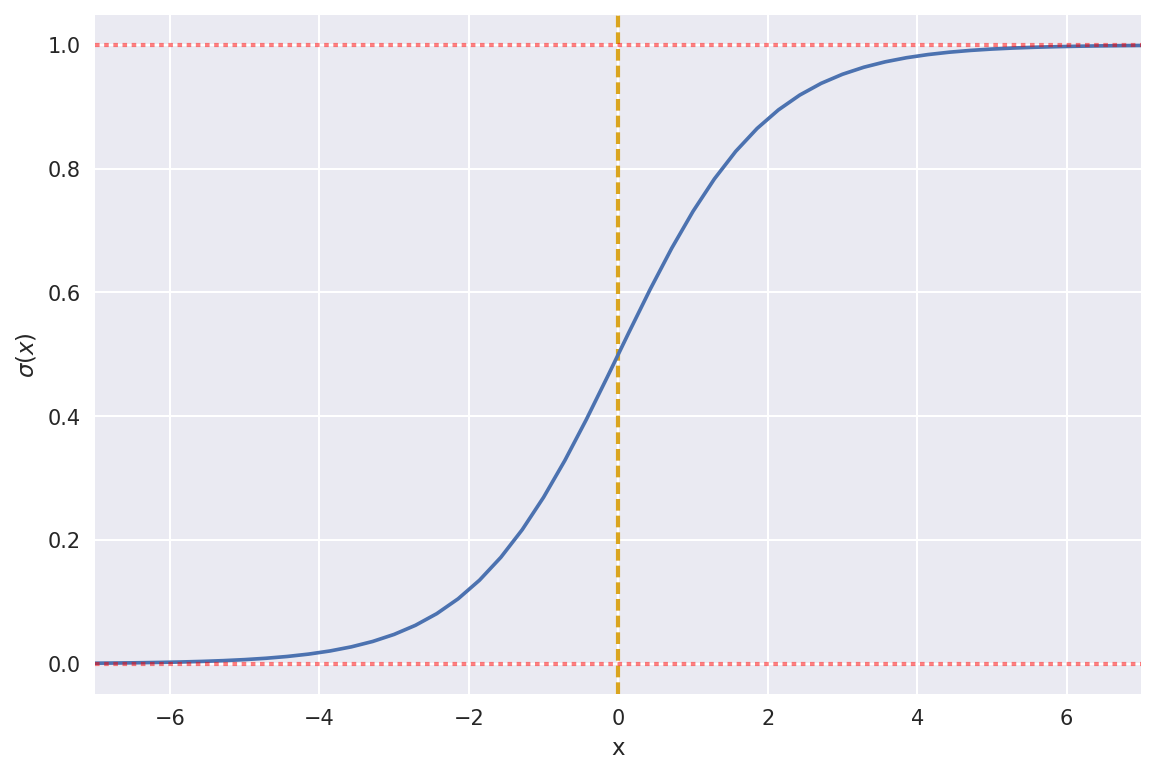
\includegraphics[height=.33\textheight]{figures/sigmoid.png}
\caption{The standard logistic sigmoid function $y = \sigma(x)$}
\label{fig:sigmoid}
\end{figure}

This probability is used for estimating the value of $y$, namely as defined in \cref{eq:probit}.

\begin{equation}
\label{eq:probit}
\begin{aligned}
	P \left( y_i = 1 \mid X \right) &= \sigma \left( X_i \beta \right) \\
	P \left( y_i = 0 \mid X \right) &= 1 - \sigma \left( X_i \beta \right)
\end{aligned}
\end{equation}

The inverse of the \emph{Logistic Function}, referred to as the \emph{Logit Function}, gives the logarithm of the \emph{Odds} of a certain element belonging to some category.

\begin{equation}
\label{eq:logit}
	\logit \left( x \right) = \log \left( \frac{\sigma \left( x \right)}{1 - \sigma \left( x \right)} \right)
\end{equation}

The logit model says that the vector $y$ is independent given the matrix $X$~\cite{freedman2009statistical}, and can be considered as inverse of the probability defined in \cref{eq:probit}.

\begin{equation}
\label{eq:prob_logit}
	\logit P \left( y_i = 1 \mid X \right) = X_i \beta
\end{equation}

The regression is usually calculated using \emph{Maximum Likelihood Estimation}~\cite{fan2008liblinear} and, unlike the estimation of the \emph{Linear Regression} presented in \cref{subsec:linearregression}, it's not possible to find a closed form expression of the coefficients that maximize the value of the likelihood function. Instead, the iterative \emph{Newton's Method} is used.

The exact formulas used to ensure fast and correct conversed used in this thesis are the ones present in \texttt{LIBLINEAR}, which is presented in~\cite{hsiastudy}.

\subsection{Decision Trees}
\label{subsec:decisiontrees}

A \emph{Decision Tree} is a decision support tool that uses a tree of decisions and their possible consequences, including change event outcomes. They are commonly used in decision analysis to help identify the most optimal strategy to reach a goal.

The tree themselves contain a root at the top, and each non-final node (including the root) contains a binary test of a certain variable; each one of these nodes contains exactly two edges connecting it to the following level, one which is followed in the case the condition is true and another for the case when the condition is false.

\begin{figure}
\centering
\includegraphicsmaybe{figures/decisiontree.png}
\caption{A decision tree, with example data that will be used later in this thesis.}
\label{fig:decision_tree}
\end{figure}

In the context of \emph{Machine Learning}, it can be used as a supervised predictive model which matches properties about the list of features $X$ to the likeliest category $y$~\cite{oded2008decisiontrees}. In the binary case, each of the final nodes contains the output label which, according to the input data, is the most probable given the result of the tests corresponding to the previous nodes to this one along with the probability of this label being true.

There are many algorithms that can generate a tree that's optimized for many different metrics. A common one is the \emph{Classification and Regression Trees (CART)} method, introduced in~\cite{breiman1993classification}, which builds the tree starting from the root and, for each non-leaf node, the variable that generates the best split according to some metric is selected~\cite{loh2011classification}. This is applied recursively until \emph{CART} detects that no further gains can be made, or some pre-set stopping rules are met.

Decision trees are prone to overfitting~\cite{oded2008decisiontrees}. Since a single tree can make an arbitrarily good classification of a set of features despite their properties (unlike models like linear regression, where the data has to be linearly separable), it can lose the capability to generalize for instances not presented in training. This occurs when the tree has too many nodes relative to the amount of training data; \Cref{fig:decisiontreeoverfitting} illustrates the overfitting process.

\begin{figure}
\centering
\includegraphicsmaybe{decisiontreeoverfitting.png}
\caption{Overfitting in decision trees. The training error starts relatively high, and it continuously declines as the tree becomes bigger. However, while the same is true of the generalization error for the first part of the graph, the error starts to increase due to overfitting}
\label{fig:decisiontreeoverfitting}
\end{figure}

A common mechanism to prevent overfitting in \emph{Decision Trees} is \emph{Pruning}, which reduces the size of decision tree by cutting sections that provide relatively little improvement of the result on the training data.

\subsection{Random Forest}
\label{subsec:randomforest}
\todo{Add Random Forest}


